\documentclass[11pt]{article}
\usepackage{amsmath,amsthm,amssymb,fullpage,graphicx,hyperref,listings}
\usepackage{listings,color,setspace}
\author{Andy Reagan}
\title{Math 337 Homework 13}

     \def\NN{\mathbb{N} }
     \def\ZZ{\mathbb{Z} }
     \def\QQ{\mathbb{Q} }
     \def\RR{\mathbb{R} }
     \def\CC{\mathbb{C} }
     \def\f{\frac }
     \def\b{\begin }
     \def\e{\end }
     \def\Log{\text{Log} \,}
     \def\Re{\text{Re} \, }
     \newcommand{\pdiff}[2]{\frac{\partial #1}{\partial #2}}
     \newcommand{\partialdiff}[2]{\frac{\partial #1}{\partial #2}}
     \newcommand{\pdiffsq}[2]{\frac{\partial^2 #1}{{\partial #2}^2}}
     \newcommand{\pdiffcu}[2]{\frac{\partial^3 #1}{{\partial #2}^3}}
     \newcommand{\pdiffhi}[3]{\frac{\partial^#3 #1}{{\partial #2}^#3}}
     \newcommand{\diff}[2]{\frac{{\rm d}#1}{{\rm d}#2}}
     \newcommand{\diffsq}[2]{\frac{{\rm d}^{2}#1}{{\rm d} {#2}^2}}
     \newcommand{\diffhi}[3]{\frac{{\rm d}^#3 #1}{{\rm d} {#2}^#3}}
     \newcommand{\tdiff}[2]{\mbox{d} #1/\mbox{d} #2}
     \newcommand{\tdiffsq}[2]{\mbox{d}^{2} #1/\mbox{d} {#2}^2}
     \newcommand{\tpdiff}[2]{\partial #1/\partial #2}
     \newcommand{\tpdiffsq}[2]{\partial^2 #1/\partial {#2}^2}
     \newcommand{\bvec}[1]{\vec{ {\bf #1 } }}
     \newcommand{\oh}[1]{O(h^{{#1}})}

\lstset{language=MATLAB,
basicstyle=\ttfamily\scriptsize\singlespacing,
keywordstyle=\color{black},
stringstyle=\color{black},
commentstyle=\color{black},
morecomment=[l][\color{black}]{\#},
frame=L,
xleftmargin=\parindent,
%%numbers=left,                   %% where to put the line-numbers
%%numberstyle=\scriptsize,      %% the size of the fonts that are used for the line-numbers
%%stepnumber=1,                   %% the step between two line-numbers. If it is 1 each line will be numbered
numbersep=5pt,
breaklines=true,        %% sets automatic line breaking
breakatwhitespace=false,    %% sets if automatic breaks should only happen at whitespace
escapeinside={\%*}{*)} 
}

\begin{document}
\maketitle

\begin{enumerate}

\item We start by writing the corresponding equation for (13.5) as 
\[ \f{U_m ^{n+1} - U_m ^{n} }{\kappa}  = \f{1}{2} \left [ a\f{U_{m+1} ^n -2 U_{m} ^n +U_{m-1} ^n}{h^2} + \f{1}{h^2} f(x_m ,t_n ) + a\f{U_{m+1} ^{n+1} -2 U_{m} ^{n+1} +U_{m-1} ^{n+1}}{h^2} + \f{1}{h^2} f(x_m ,t_{n+1} ) \right ] .\]
Since $f$ is known for all times $t$, we then have 
\[ \left (1-\f{ar\delta_x ^2 }{2}\right )U_m ^{n+1} = \left (1+\f{ar\delta_x ^2 }{2}\right )U_m ^{n} + \f{r}{2} \left ( f(x_m ,t_n ) + f(x_m ,t_{n+1} ) \right )  .\]
With $r = \kappa / h^2$, we write the above in vector notation 
\[ \left (1-\f{ar}{2}A\right )\bvec{U} ^{n+1} = \left (1+\f{ar}{2}A\right )\bvec{U} ^{n} + \bvec{b},\]
where the matrix $A$ is defined as in the notes (Eq 13.10) and $\bvec{b}$ is defined as
\[ \bvec{b} = \f{r}{2} \left ( \begin{array}{c} g_0 (t_n) + g_0(t_n+1) \\0\\.\\0\\ g_1 (t_n) + g_1(t_n+1) \end{array} \right ) + \f{r}{2} \left ( f( \bvec{x} ,t_{n+1} ) + f( \bvec{x} , t_n ) \right ) \].

\item For the $\theta$ family of methods, we have the discreization from Eq 13.16 as
\[ \bvec{U}^{n+1} = \bvec{U}^{n} + \kappa \left ( \left ( 1-\theta \right ) f(t_n, \bvec{U}^n ) + \theta f(t _{n+1},\bvec{U}^{n+1} ) \right ) \]
which leads to the method corresponding to Eq 13.17, which is
\[ (I-r\theta A) \bvec{U}^{n+1} = (I +r (1-\theta) A)\bvec{U}^n + \bvec{b}.\]
Following the traditional stability analysis, Eq 13.20 writes this in a form more suitable for the stability analysis (where we've dropped $\bvec{b}$ since we only need the homogeneous problem):
\[ \bvec{U}^{n+1} = (I-r\theta A) ^{-1} (I +r (1-\theta) A)\bvec{U}^n .\]
Writing this again for each node, we have
\[ (1-r\theta \partial _x ^2 ) U^{n+1} _m  =  (1 +r (1-\theta) \partial _x ^2 )U^n_m  .\]
Expanding,
\[ U^{n+1} _m-r\theta (U^{n+1} _{m+1} -2U^{n+1} _m + U^{n+1} _{m-1} )  =   U^n_{m}+r (1-\theta) (U^n_{m+1}-2U^n_{m}+U^n_{m})  .\]
Since this equation is linear, the error also obeys this difference scheme, and we write
\[ \epsilon^{n+1} _m-r\theta (\epsilon^{n+1} _{m+1} -2\epsilon^{n+1} _m + \epsilon^{n+1} _{m-1} )  =   \epsilon^n_{m}+r (1-\theta) (\epsilon^n_{m+1}-2\epsilon^n_{m}+\epsilon^n_{m})  .\]
Using the same Fourier expansions as in Chapter 12 of the notes (and my Homework 12), we have
\begin{align*} &\rho^{n+1} e^{i \beta m h}-r\theta (\rho ^{n+1} e^{i \beta (m+1) h} -2\rho ^{n+1} e^{i \beta m h}+ \rho ^{n+1} e^{i \beta (m-1) h} )\\  ~~~~~~&=   \rho ^{n} e^{i \beta m h}+r (1-\theta) (\rho ^{n} e^{i \beta (m+1) h}-2\rho ^{n} e^{i \beta m h}+\rho ^{n} e^{i \beta (m-1) h})  .\end{align*}
Cancelling the common $\rho ^n e^{i\beta mh}$ we are left with
\begin{align*} \rho -r\theta (\rho e^{i \beta h} -2\rho + \rho e^{-i \beta h} ) =   1+r (1-\theta) (e^{i \beta h}-2+ e^{-i \beta h})  .\end{align*}
Letting $z = -4r \sin ^2 \left ( \f{\beta h }{2} \right )$ we have
\begin{align*} \rho (1-\theta z) =   1+ (1-\theta) z, \end{align*}
and therefore
\begin{align*} \rho  =  \f{ 1+ (1-\theta) z} {1-\theta z}. \end{align*}
For stability we require $|\rho| < 1$ and so 
\begin{align*} &\left | \f{ 1+ (1-\theta) z} {1-\theta z} \right | < 1\\
-1 & < \f{1+ (1-\theta) z  }{1-\theta z}  < 1 \\
-1+\theta z & < 1+ (1-\theta) z < 1-\theta z \\
-2+\theta z & < z-\theta z < -\theta z \\
-2+2\theta z & < z < 0 \end{align*}
Since $z<0$ always, ($\sin^2 \in [0,1]$ and $r>0$), we now deal with:
\begin{align*} -2& < (1-2\theta) \left ( -4r \sin ^2 \left (\f{\beta h}{2} \right ) \right )\\
\f{1}{2} & > (1-2\theta) r \sin ^2 \left (\f{\beta h}{2} \right )\end{align*}
Since again $\sin ^2 \left (\f{\beta h}{2} \right ) \in [0,1]$, for the above to hold for any value of $\beta h$, we have 
\[  (1-2\theta) r < \f{1}{2}, \]
which is the same as Eq 13.27.


\item Let $\vec{v}$ be an eigenvector of $A$.
Therefore $\exists \lambda $ such that
\[A\vec{v} = \lambda \vec{v},\]
and clearly multiplying by any scalar $a$ we have
\[aA\vec{v} = a\lambda \vec{v}.\]

Also, notice that 
\[ I\vec{v} = \vec{v} = 1\cdot \vec{v} \]
where by $\cdot$ scalar mutliplication is implied.
The above equation can then, be multiplied by any scalar $b$.
Adding the two previous equations, we have
\begin{align*} aA\vec{v} bI\vec{v}  &= a\lambda \vec{v} + b\vec{v}\\ \vspace{1mm}
\Rightarrow (aA+ bI)\vec{v}  &= (a\lambda +b) \vec{v}\end{align*}
which proves that $a\lambda +b$ is an eigenvalue of $aA+ bI$ with eigenvector $\vec{v}$.

In the above derivation, replacing $a \to c, b \to d$ we have
\[ (cA+ dI)\vec{v} = (c\lambda +d) \vec{v}.\]
Taking the inverse of both sides, we have
\[ (cA+ dI)^{-1}\vec{v} = (c\lambda +d)^{-1} \vec{v},\]
which proves that $(c\lambda +d)^{-1}$ is an eigenvalue of $(cA+ dI)^{-1}$ with eigenvector $\vec{v}$.

Finally, in Eq 13.20
\[ \bvec{U} ^{n+1}  = (I - r \theta A ) ^{-1} (I + r(1-\theta ) A) \bvec{U} ^n \]
let $a = r(1-\theta) , b = 1, c = -r\theta, $  and $d=1$.
Therefore the eigenvalues of 
\[ \mathcal{M} =  (I - r \theta A ) ^{-1} (I + r(1-\theta ) A) \]
for $\lambda _j$ an eigenvalue of $A$ are
\[ (a \lambda _j + b) (c\lambda _j + d) ^{-1}  = \f{1 + r(1-\theta) \lambda _j }{1 - r\theta \lambda _j}. \]

\item 

%% \lstinputlisting[language=Matlab]{andy_hw13_prb04.m}

%% \begin{figure}[h!]
%%   \centering
%%     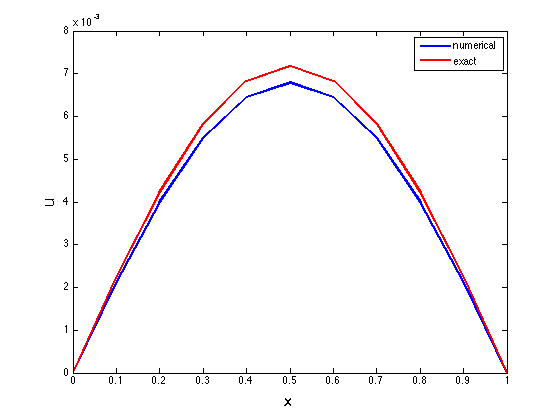
\includegraphics[width=0.45\textwidth]{andy_hw12_prb01_02.png}
%%   \caption{The numerical and exact solution for $h=0.1$.}
%% \end{figure}

\end{enumerate}

\end{document}



